\chapter{System test and optimization}
\section{Test setup}
During test of the system we choose two paths. One was optimization of clocks and hereby how responsive our system could be. This test will hereafter be called "System clocks".\\
The other test is precision test. How precise can the system measure distance. This test will hereafter be called "Full system test".\\
\subsection{System clocks}
The amount of clocks used by our system is a pointer for how efficient the system is and how much time it takes for the system to run. To find the system clocks add -DDO$\_$CYCLE$\_$COUNTS to the compiler. Add the following code:\\
\begin{lstlisting}
cycle_t start_count;
cycle_t stop_count;
	
START_CYCLE_COUNT(start_count);
>> your code <<
STOP_CYCLE_COUNT(stop_count, start_count);
\end{lstlisting}
After this we can read the clock count and hereby determine the efficiency.
\subsection{Full system test}
The setup consists of 2 speakers, a microphone and a blackfin bf533 kit connect to a computer running VisualDSP++. One of the speakers is connected to the blackfins left audioport0 and one is connected to the right audioport0. The microphone is connected to the blackfins left inputport0. 

\section{Test procedure}
\subsection{System clocks}
Run the program in the VisualDSP++ debugger and put a breakpoint after the STOP part of the cycle counter. Read the cycles with:
\begin{verbatim}
View -> Debug Windows -> Locals
\end{verbatim}
\subsection{Full system test}
A piece of wood is placed at fixed intervals in front of the system. These intervals are in millimetres: 250, 500, 750, 1000, 1250, 1500, 1750, 2000, 2250, 2500. The output is found in the VisualDSP++ debugger by placing a breakpoint after measuring distance. All distances and corresponding measurement is noted.
\section{Test results}
\subsection{system clocks}
Below is listed the results from the system clocks test.
\begin{table}[H]
\centering
    \begin{tabular}{|l|l|}
    \hline
    Variable           & Clock Cycles (mm) \\ \hline
    start$\_$count        & 1385380           \\ \hline
    stop$\_$count         & 285290476         \\ \hline
    Program total      & 283905096         \\ \hline
    \end{tabular}
    \caption{System clocks results}
\end{table}
\subsection{Full system test}
Below is listed the results from the full system test.
\begin{table}[H]
\centering
    \begin{tabular}{|l|l|}
    \hline
    Real Distance (mm) & Measured Distance (mm) \\ \hline
    250                & 699                    \\ \hline
    500                & 853                    \\ \hline
    750                & 1104                   \\ \hline
    1000               & 1267                   \\ \hline
    1250               & 1579                   \\ \hline
    1500               & 1859                   \\ \hline
    1750               & 2026                   \\ \hline
    2000               & 2132                   \\ \hline
    2250               & 2434                   \\ \hline
    2500               & 2801                   \\ \hline
    \end{tabular}
    \caption{Full system test results}
\end{table}
\section{Optimization}
\subsection{Optimization of distance calculation}
As seen in the results of the full system test it is clear that there exists some kind of offset and a sensitivity drift. Below is a plot of the distances measured compared to the real distance:\\
\begin{figure}[H]
\centering
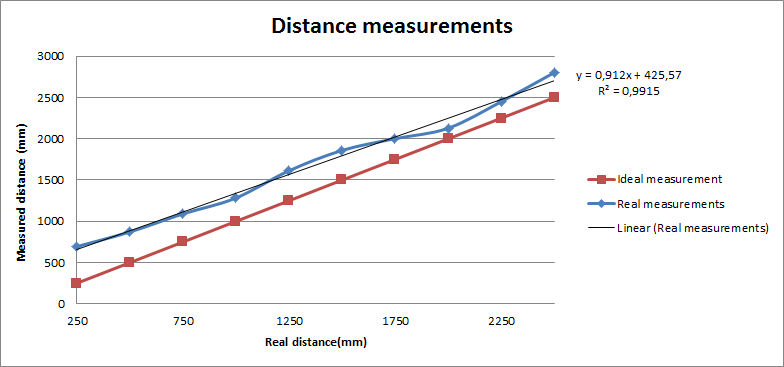
\includegraphics[width=0.95\textwidth]{billeder/first_test_results_graph}
\caption{Distance performance graph}
\end{figure}
The tendency line plotted in excels shows how much off we are since the function for the graph should have been y=1x. Therefore we need to find what values to subtract and divide from our measurements to calibrate our system. The function is found to be:\\
\begin{equation}
Calibrated_{meas}=1.095*Original_{meas}-426
\end{equation}
These values are implemented in the system and another iteration of test is performed.\\
\section{Optimized test results}
The results found in this chapter are from tests done the same way as previously except with the system optimized.
\subsection{Full system test}
\begin{table}[H]
\centering
    \begin{tabular}{|l|l|}
    \hline
    Real Distance (mm) & Measured Distance (mm) \\ \hline
    250                & 210                   \\ \hline
    500                & 462                    \\ \hline
    750                & 654                   \\ \hline
    1000               & 1075                   \\ \hline
    1250               & 1244                   \\ \hline
    1500               & 1671                   \\ \hline
    1750               & 1756                   \\ \hline
    2000               & 2034                   \\ \hline
    2250               & 2316                   \\ \hline
    2500               & 2528                   \\ \hline
    \end{tabular}
    \caption{Full system test results with optimized precision}
\end{table}
To visualize the improvement a similar graph as from optimization is made to compare the new results with the old.\\
\begin{figure}[H]
\centering
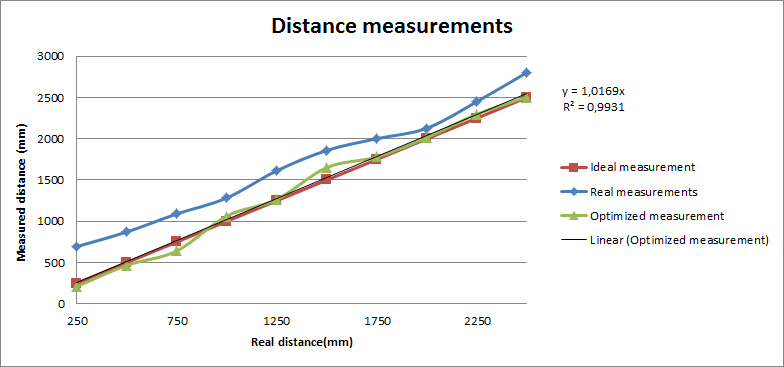
\includegraphics[width=0.95\textwidth]{billeder/first_test_results_graph_optimized}
\caption{Distance performance graph optimized}
\end{figure}
Obviously the results has been improved a lot. The reason for the constant offset of the 42cm is due to group delay on the blackfin board.\\
The optimization made isn't much of a perfomance issue since the blackin dsp is made to perform multiplication and addition tasks.\\
\section{Averaging of distance}
While making all the test we did we noticed the output frequency generated based on the measured distance wasn't always stationary. We wanted to fix this and therefore implemented an averaging algorithm. The least recourse consuming averaging we knew of was the exponential averaging filter. Below is a sketch of how it works.\\
\begin{figure}[H]
\centering
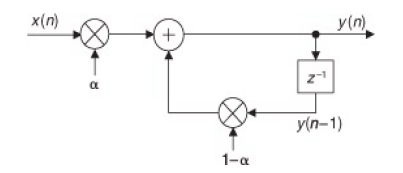
\includegraphics[width=.5\textwidth]{billeder/exp_avg}
\caption{Exponential averaging filter}
\end{figure}
The figure is from the book "Understanding Digital Signal Processing" by Richard G- Lyons. As illustrated in the figure it multiplies the current sample with the alpha filter coefficient, it then multiplies the last sample ($Z^{-1}$) with 1-alpha. This effectively  weight the samples with alpha and hereby the "weight" of the old samples still effects the outcome (depending on the alpha value) several samples after it has been used.\\
Using "trial \& error" we found an alpha value of 0.2. An alpha of this size means a somewhat significant averaging since we only use .2 of every new sample and .8 of the old calculated value.\\
We then tested how responsive the system was to distance change. Looking at the average the filter actually takes the exact same number of samples each time to settle at a specific distance, namely around 10-12 samples. In our system it meant around 1 second which we found sufficient.\\
Below is 30 samples in a row showing the settling of a distance measurement to a fixed distance of 1250 mm.\\
\begin{figure}[H]
\centering
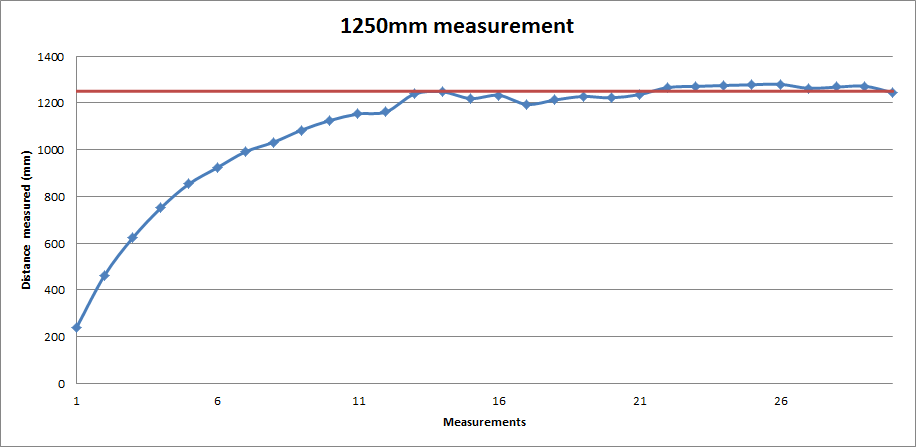
\includegraphics[width=0.9\textwidth]{billeder/avg_chart}
\caption{Chart showing exponential averaging filter}
\end{figure}